\documentclass[11pt]{amsart}
\usepackage{geometry}                % See geometry.pdf to learn the layout options. There are lots.
\geometry{letterpaper}                   % ... or a4paper or a5paper or ... 
%\geometry{landscape}                % Activate for for rotated page geometry
%\usepackage[parfill]{parskip}    % Activate to begin paragraphs with an empty line rather than an indent
\usepackage{graphicx}
\usepackage{amssymb}
\usepackage{epstopdf}
\DeclareGraphicsRule{.tif}{png}{.png}{`convert #1 `dirname #1`/`basename #1 .tif`.png}

\usepackage{amsmath}
\usepackage{algorithm}
\usepackage[noend]{algpseudocode}

\makeatletter
\def\BState{\State\hskip-\ALG@thistlm}
\makeatother

\title{KD-tree}
%\author{The Author}
%\date{}                                           % Activate to display a given date or no date

\begin{document}
\maketitle
%\section{}
%\subsection{}

\section{Introduction}
This document describes the solution details of KD-tree project. In Section~\ref{sec:basic_components} we describe the basic data structures and components used in the project. In Section~\ref{sec:algorithms} we describe the algorithms used to build and search KD-trees. In Section~\ref{sec:implementation} we describe some of the design decisions we made during this project. We conclude the document by describing some of the potential improvements we could have done in this project.

\section{Basic components}
\label{sec:basic_components}

The various components used in this project are as follows:

\begin{list}{\labelitemi}{\leftmargin= 1.4cm} \setlength\itemsep{1em}

\item \textbf{Sample matrix}: Input samples are represented as a matrix $M \in R^{m \times n}$, where we have $m$ samples and $n$ dimensions and $M_{ij}$ represents the value for $i^{th}$ sample in $j^{th}$ dimension. We use Eigen library \cite{Guennebaud:2010aa} to represent this matrix.

\item \textbf{Segment}: Segment is the logical partitioning of samples that is used by the KD-tree algorithm during tree construction. An example of segments is shown in Figure \ref{fig:segment}. The six samples are stored in memory as an Eigen matrix and shared by all segments. Each segment contains a vector of sample ids that are present in the segment. The first segment contains all the sample ids. 

After a split, during tree building process, we get two almost equal segments which contain a reference to the main matrix and have a vector of sample ids that indicate the samples from matrix which belong in the segment. Partitioning samples this way allows us to develop recursive or parallel algorithms to build trees efficiently. 

\begin{figure}[t!]
\centering
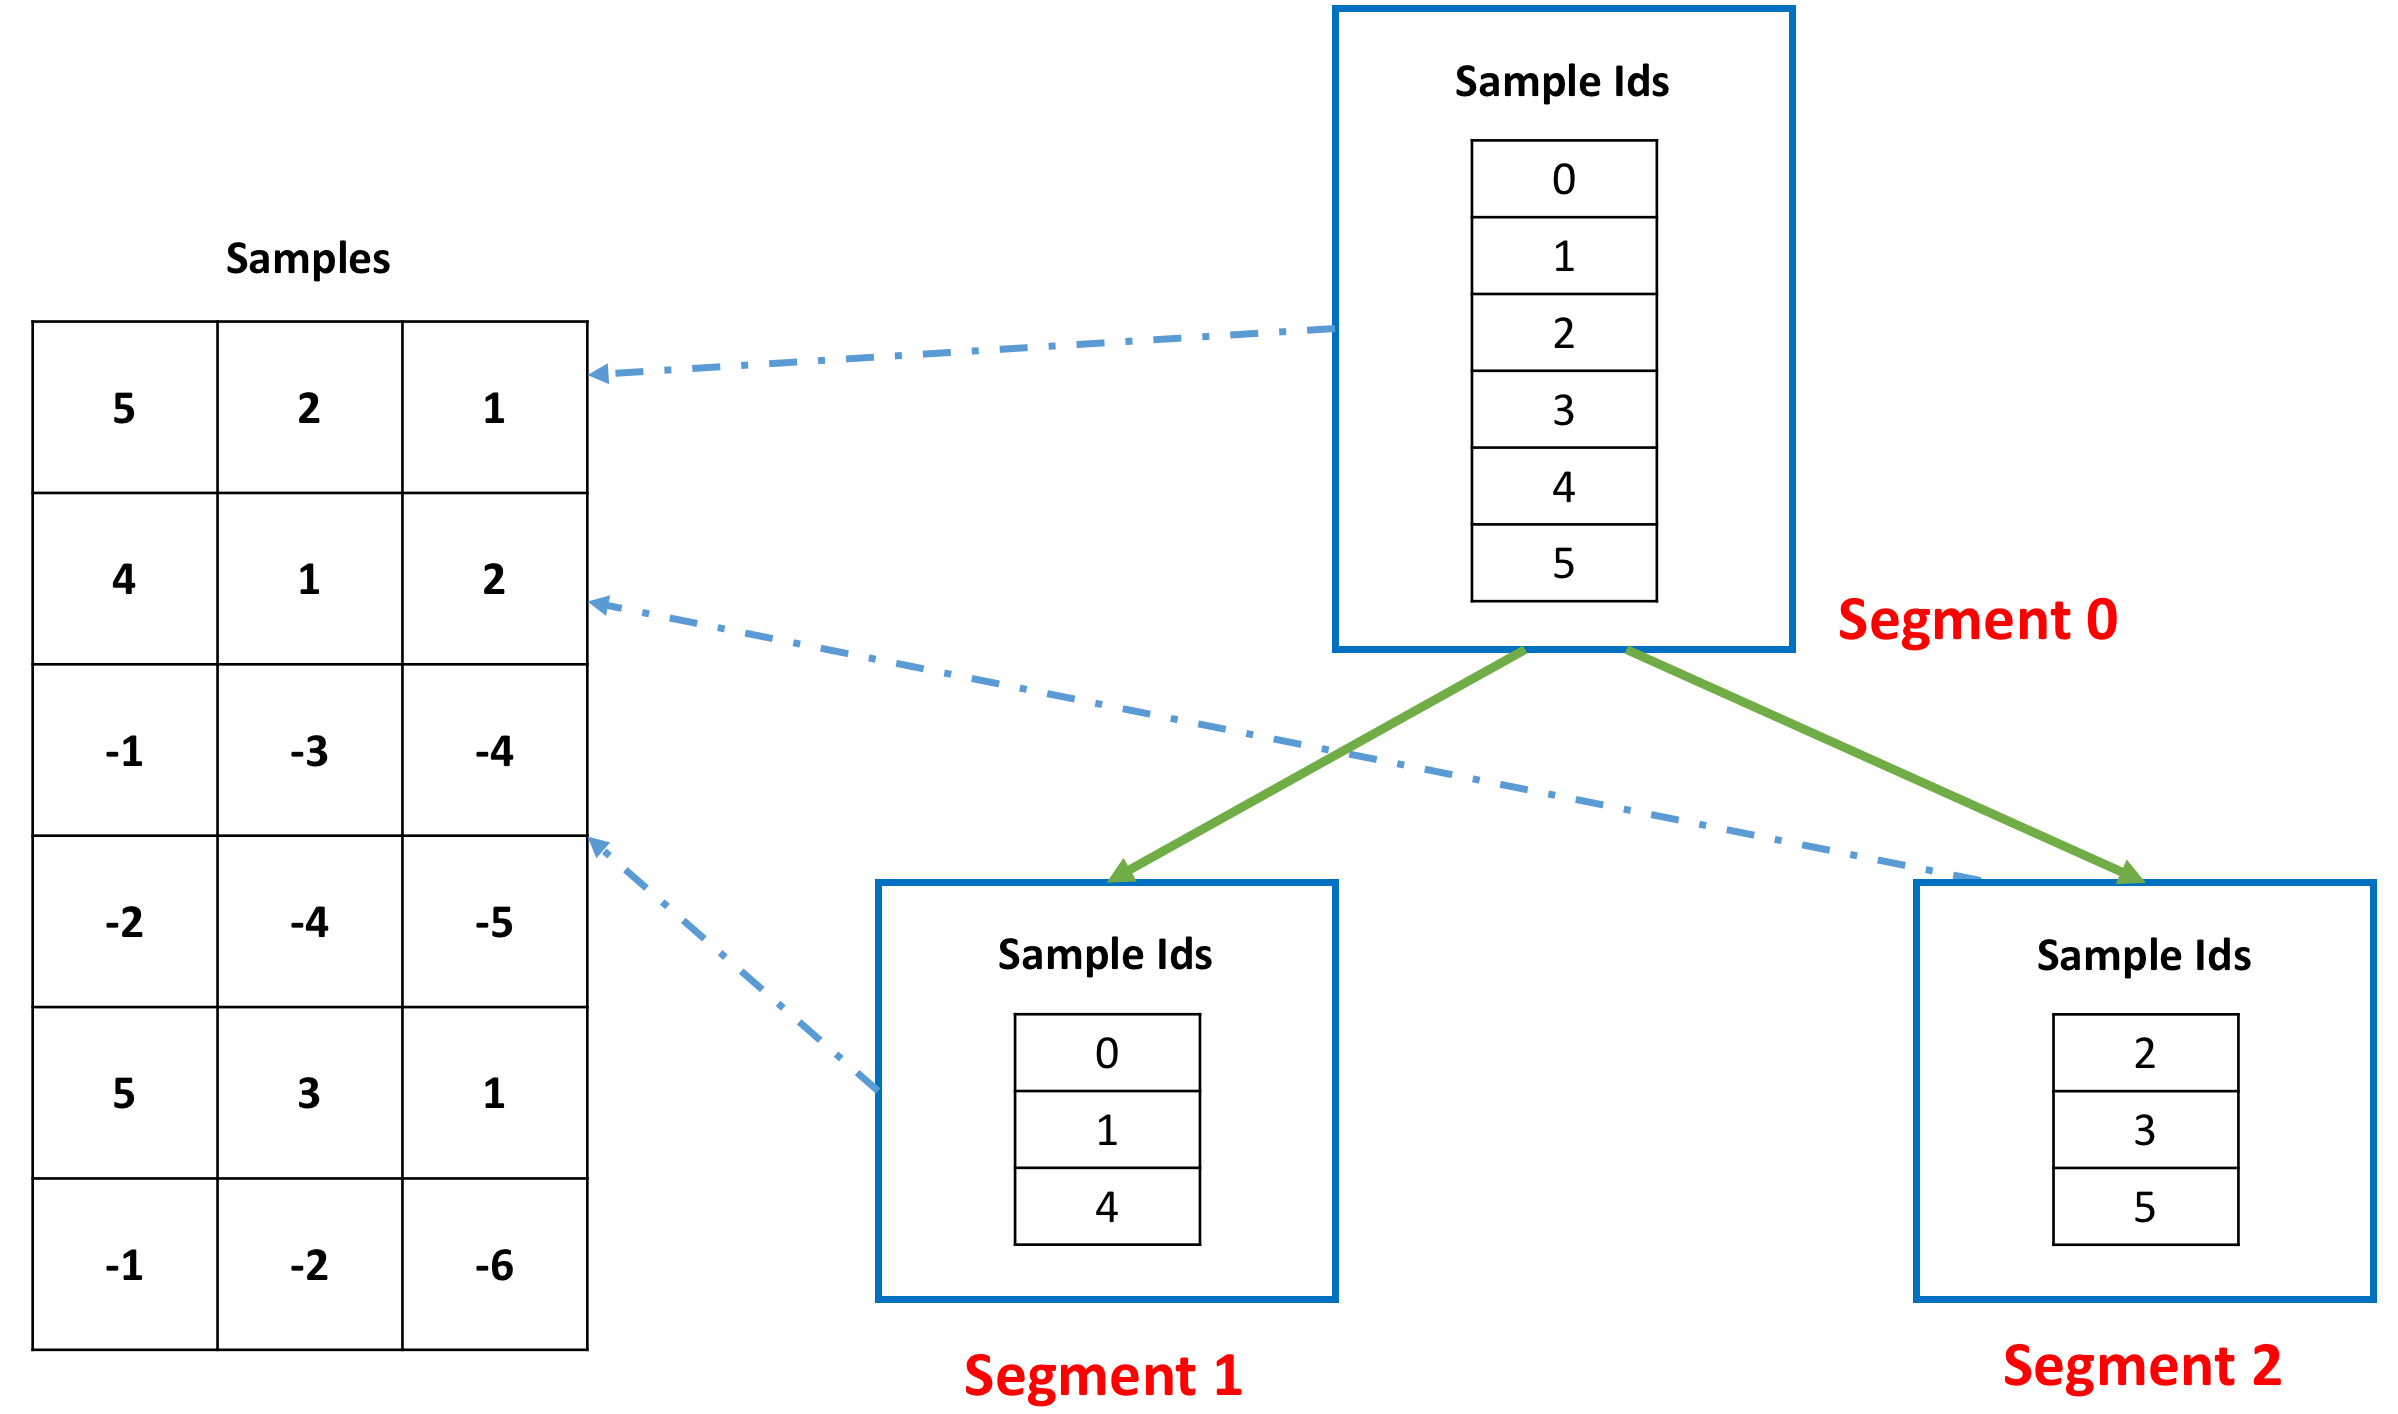
\includegraphics[width=\linewidth]{images/segment}
\caption{Example of how samples are stored in an Eigen matrix and then shared between segments.}
\label{fig:segment}
\end{figure}

\begin{figure}[t!]
\centering
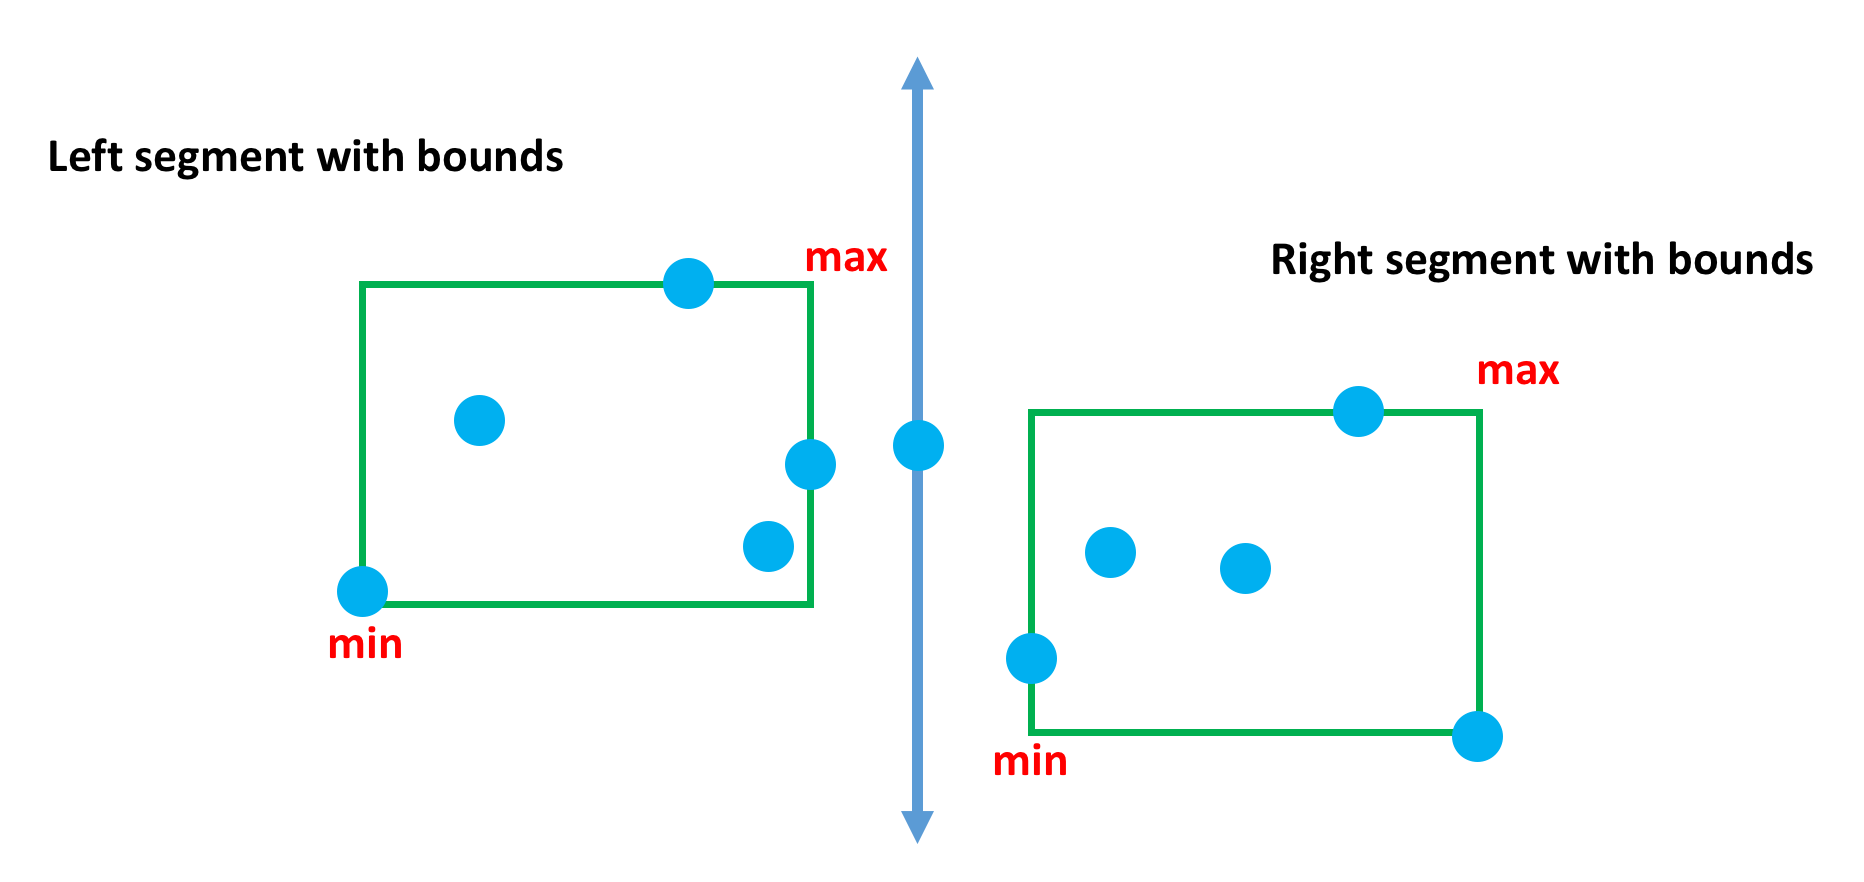
\includegraphics[width=\linewidth]{images/bounding_box}
\caption{Example of a split, with split point, left and right bounding boxes.}
\label{fig:bounding_box}
\end{figure}


\item \textbf{Split}: This contains the information that we need to split samples into segments. This is created during tree building process and used when we are searching for a query in the tree. Every internal node in the tree contains this split object. Split contains the following details (Figure \ref{fig:bounding_box}):
\vspace{1.5 mm}
\begin{enumerate} \setlength\itemsep{0.5em}
\item Split dimension ($d_{t+1}$): This the dimension along which we will be splitting the samples at ${(t+1)}^{th}$ node during the search.
\item Split point: This is the point that is used to split the samples in the segment into almost equal size. If the number of points in the segment are odd then the split point is the one in middle otherwise, it is the average of the 2 points in the middle. This is the point in the center of Figure  \ref{fig:bounding_box}.
\item Bounds:  These define the boundaries of left and right segments generated after the current segment is split. We store: (i) min point, which is the min value in all dimensions for samples in the segment; and, (ii) max point, which is the max value in all dimensions for samples in the segment.
\end{enumerate}
\item \textbf{Split Dimension Selector}: This is used to select the dimension that will be used to split the samples next. The selector supports 2 methods:
\vspace{1.5 mm}
\begin{enumerate}\setlength\itemsep{0.5em}
\item Cycle through axis: This method cycles through dimensions. 
\[ d_{t+1} = (d_{t} + 1)  \% n \]
\item Highest range axis: This method selects a dimension that has the maximum spread of points.
\[ d_{t+1} = \operatorname{arg\,max}_j  (\text{max\_value\_along j - min\_value\_along j})\] 
\end{enumerate}

\item \textbf{Split Point Selector}: This is used to select the threshold that will be used to separate points. These methods return the same value but the complexity of finding them is different depending on the method. This selector supports 2 methods:
\vspace{1.5 mm}
\begin{enumerate}\setlength\itemsep{0.5em}
\item Median: Sorts the values for dimensions we are splitting across and picks the median. This has a complexity of $O(nlogn)$. 
\item Median \-of \-median: This uses a selection algorithm that picks the $k^{th}$ biggest item with $O(n)$ complexity.
\end{enumerate}

\item \textbf{KD-tree}: The KD-tree object is represented as an array of nodes. A node can either be an  internal node containing information of how to split samples or a leaf node that contains id for a sample. The array is indexed from 0, so for internal nodes at index $k$, the left child is at $2k + 1$ and the right child is at $2k + 2$.

\end{list}

\section{Algorithms}
\label{sec:algorithms}
I implemented three algorithms in this project. First two of them are related to building KD-tree and the third one is about searching a query in the tree. Of the two tree-building algorithms one uses recursion (Algorithm~\ref{tree_building_recursive}) and another one is a parallel (Algorithm~\ref{tree_building_parallel}). The third algorithm is used to search for a query in a KD-tree (Algorithm~\ref{query_searching}). The details are as follows:

\begin{list}{\labelitemi}{\leftmargin= 1.4cm} \setlength\itemsep{1em}
%\vspace{5 mm}
\item\textbf{Recursive tree building algorithm}:  We first load samples into an Eigen matrix and then initialize KD-tree as an array of nodes. We then create a big segment containing all the samples and call the function  to build the tree. This recursive function gets the dimension to split by and splits the big segment into 2 segments of almost equal parts using the split point. It inserts the split point into KD-tree and then calls the recursive function again with the smaller segments. If the segment contains just one sample then the function inserts a leaf node with that segment into the tree.

\begin{algorithm}[!t]
\caption{Tree building algorithm (recursive)}
\label{tree_building_recursive}
\begin{algorithmic}[1]
\State Load samples
\State Initialize KD-tree as an array of nodes of size $2^{\left \lfloor{log_{2}(\text{num samples})}\right \rfloor + 1 }$ 
\State Create Segment $S_0$ which contains all samples
\State 
\State BuildTreeRecursive($S_0$)
\State 
\Procedure{BuildTreeRecursive}{Segment S}
\If {S contains just one sample} 
\State Create a leaf node with one sample and insert it to the KD-tree
\Else
\State Get dimension to split by using dimension selector.
\State Get the split threshold using split point selector.
\State Insert an internal node with split information into KD-tree.
\State
\State Generate the segments:
\State $S_l \gets $ all samples less than split threshold; and
\State $S_r \gets $  all samples greater than the split threshold
\State
\State BuildTreeRecursive($S_l$)
\State BuildTreeRecursive($S_r$)
\EndIf
\EndProcedure
\end{algorithmic}
\end{algorithm}


%\vspace{5 mm}
\item\textbf{Parallel tree building algorithm}: This is similar to the recursive algorithm in terms of functionality but doesn't have the additional overhead of maintaining system stack during recursion. Instead, it uses a thread-safe queue that can be used like a stack. In addition to this, the algorithm is multithreaded which allows for faster tree building on a big dataset when enough resources are available.

\begin{algorithm}[!t]
\caption{Tree building algorithm (parallel)}
\label{tree_building_parallel}
\begin{algorithmic}[1]
\State Load samples
\State Initialize KD-tree as an array of nodes of size $2^{\left \lfloor{log_{2}(\text{num samples})}\right \rfloor + 1 }$ 
\State Create Segment $S_0$ which contains all samples
\State 
\State BuildTreeParallel($S_0$)
\State
\Procedure{BuildTreeParallel}{Segment S}
\State Create a thread pool $P$
\State Initialize a thread-safe queue Q
\State Push segment onto queue: $Q \gets Q + S$
\While {Q is not empty}
\State $p \gets \text{next free thread in P}$
\State $S_c \gets \text{Last item from } Q$ \hspace{0.5in}// mimics stack
\State $p \rightarrow$  ProcessSegment($S_c$, $Q$)
\EndWhile
\EndProcedure
\State
\Procedure{ProcessSegment}{Segment S, Queue Q}
\If {S contains just one sample} 
\State Create a leaf node with one sample and insert it to the KD-tree
\Else
\State Get dimension to split by using dimension selector.
\State Get the split threshold using split point selector.
\State Insert an internal node with split information into KD-tree.
\State
\State Generate the segments:
\State $S_l \gets $ all samples less than split threshold; and
\State $S_r \gets $  all samples greater than the split threshold
\State
\State $Q \gets Q + S_r$
\State $Q \gets Q + S_l$
\EndIf
\EndProcedure
\State 
\end{algorithmic}
\end{algorithm}

%\vspace{5 mm}
\item\textbf{Query search algorithm}: This algorithm is used to search for a query in a KD-tree. Like the iterative (parallel) version, this uses a stack to track the sample space that needs to be explored. We start by loading the samples on which the tree was built and the KD-tree. We then initialize the stack with the root node of KD-tree. In addition to this, we also initialize 2 variables - the nearest neighbor discovered so far during the search and the euclidian distance from it. The nearest neighbor is initialized to the first node and its distance is set to Infinity. We then start the search until the stack is empty. During the search, if we reach the leaf node, we check if the sample at that node is closer than the nearest neighbor found so far. If it is, we update the nearest neighbor and the distance from it.

An important aspect of this search algorithm is the approach used to find the distance between the query and the bounds identified during the KD-tree building process. A bound is represented using 2 points $(point_{min}, point_{max})$, where $point_{min}$ and $point_{max}$ and $n$-dimensional vectors, similar to query $q$. The split distance between the two is defined as follows:
\[ d(i) =
  \begin{cases}
    point_{min}[i] > q[i]       & \quad (point_{min}[i] - q[i])\\
    point_{max}[i] < q[i]       & \quad (q[i] - point_{max}[i]) \\
    otherwise                      & \quad 0
  \end{cases}
\]
\[distance(bound, q) =  \sum_{i = 0}^{n-1} d(i)^{2}\]

\begin{figure}[t!]
\centering
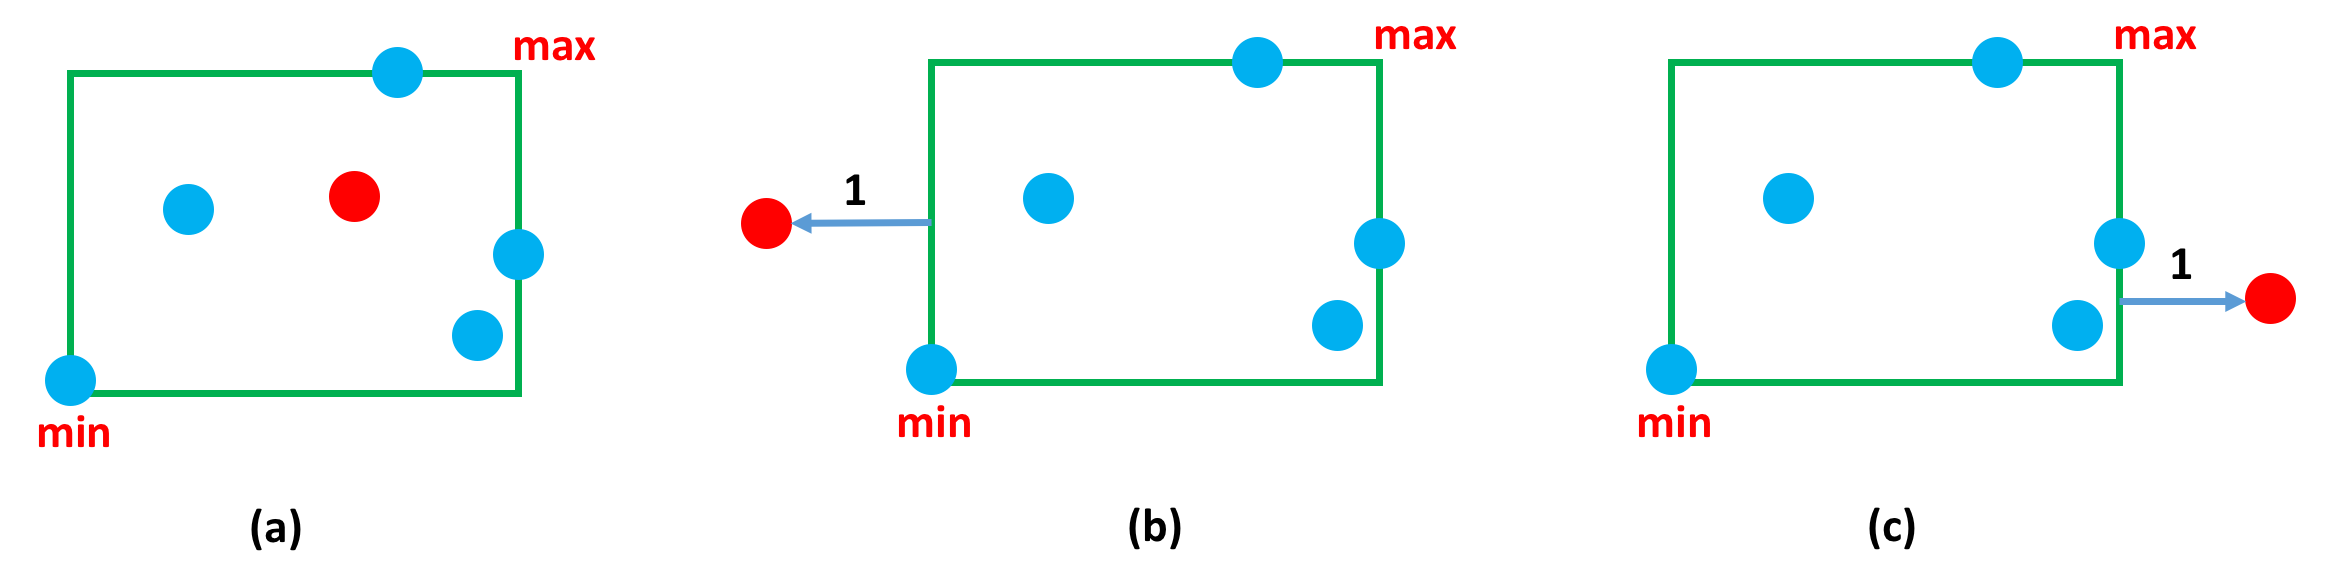
\includegraphics[width=\linewidth]{images/bound_distance}
\caption{An example of a distance between query (red point) and the bounding box is shown. Case (a) has the query inside the bound so it has a distance of 0. In case (b) and (c) the query is about $1$ unit away from the bounding box. Hence, is at a distance of 1.}
\label{fig:bound_distance}
\end{figure}

This function keeps the distance between two points to be 0 if they are within the range otherwise we add the squared distance from the region. This is similar to the approach discussed in \cite{bounding_distance}.  An example of this is shown in Figure~\ref{fig:bound_distance}. Using this definition of distance, the search algorithm continues to decide if a branch needs to be explored in the search tree.
\end{list}

\begin{algorithm}[!t]
\caption{Query searching algorithm}
\label{query_searching}
\begin{algorithmic}[1]
\State Load samples
\State Load KD-tree as an array of nodes
\State
\Procedure{SearchQuery}{Query q}
\State $N \gets \text{First node in KD-tree}$
\State Push node onto queue: $Q \gets Q + N$
\State
\State Initialize current nearest neighbor $N^\prime$ and Euclidean distance from that neighbor $d^\prime$
\State $N^\prime \gets N$
\State $d^\prime \gets \infty$
\State
\While {Q is not empty}
\State $N_i \gets \text{Last item from } Q$ \hspace{0.5in}// mimics stack
\If {$N_i$ is a leaf node} 
\State $d \gets distance(N_i, q)$
\If {$d \leq d^\prime$}
\State $d^\prime \gets d$
\State $N^\prime \gets N_i$
\EndIf
\Else
\State Get current split: $P \gets N.split$
\State $d_{left} \gets distance(P.leftBounds,\text{ } q)$ 
\State $d_{right} \gets distance(P.rightBounds,\text{ } q)$ 
\State
\State $leftIsCloser \gets d_{left} \leq d^\prime$ 
\State $rightIsCloser \gets d_{right}  \leq d^\prime$ 
\State
\If {$leftIsCloser$ \&\& $rightIsCloser$} 
\State Order in which to explore next side is decided by which is the closer side.
\If { $d_{left} \leq d_{right}$}
\State $Q \gets Q + P.rightNode$
\State $Q \gets Q + P.leftNode$
\Else
\State $Q \gets Q + P.leftNode$
\State $Q \gets Q + P.rightNode$
\EndIf
\ElsIf {$leftIsCloser$} 
\State $Q \gets Q + P.leftNode$
\ElsIf {$rightIsCloser$} 
\State $Q \gets Q + P.rightNode$
\EndIf
\EndIf
\EndWhile
\EndProcedure
\end{algorithmic}
\end{algorithm}


\section{Implementation/Design}
\label{sec:implementation}

I made the following design decisions during the implementation of the algorithms.

\begin{list}{\labelitemi}{\leftmargin= 1.4cm} \setlength\itemsep{1em}

\item \textbf{Functional design}: During the design of classes I tried to follow the concepts of functional programming as much as possible. This decision allowed me to reuse code that was used to implement recursion based solution to a mutli-threaded one. It also allowed me to test different components in a modular way resulting in cleaner code and isolation of issues. I achieved functional aspects by making most of my classes immutable, i.e, the class attributes are all private and cannot be changed once they are created. The attributes are available, only if needed, through getter methods. In addition to immutable classes I made sure all the functions are pure, i.e, the value returned by the function is just dependent on the input parameters to the function and not any variables outside of it.

\item \textbf{Test driven development}: I took a test-driven approach while implementing the modules, which mean any module that I added was  thoroughly unit tested. Anytime there were dependencies between the modules I was able to test them by mocking (not gmock) the other modules. I also wrote integration tests to test the end-to-end correctness of the implementation. The datasets for the integration tests were generated using a python script, where the samples to build the tree and queries were generated randomly and the labeled data was generated by doing a $n^2$ search find the nearest neighbor and the distance from the neighbor. I then verified the correctness of my implementation by checking we are able to find nearest neighbors correctly (KDTreeHandlerTest.cpp). 

\item \textbf{Storing sample ids instead of samples}: In the built model, I decided to keep just the sample ids instead of the entire sample. From an implementation point of view either option was viable but I decided to keep just the sample ids as it avoids duplication of samples. The drawback of this approach is that the samples dataset is tied to the model.

\item \textbf{Squared distance instead of Euclidean}: In the query search algorithm I use squared distance to maintain the nearest neighbor discovered so far instead of Euclidean distance. I use Euclidean distance only in the final step while writing the results. I did this as squared distance metric doesn't change the ordering of the nearest neighbors and is computationally faster as it doesn't have to calculate the square-root required in the Euclidean distance. This is similar to the approach taken in KD-tree in scikit-learn \cite{sklearn_api}.

\end{list}

\section{Implementation/Design}
\label{sec:conclusion}
In this document I described the various data structures and components, the algorithms used to build and search KD-trees and some of the design decisions I made during the project. If I had more time, I would have liked to do the following things:
\begin{list}{\labelitemi}{\leftmargin= 1.4cm} \setlength\itemsep{1em}
\item \textbf{Store multiple samples in leaf nodes}: Right now the KD-tree continues to build the tree until leaf contains just one sample. Alternatively, we can stop the iteration when we have reached a threshold, for example, stop building tree when a node contains 10 samples. During the search process we can then do a linear search of the 10 samples to find the nearest neighbor. This can be implemented in my design without too many changes.
\item \textbf{Evaluation of parallel algorithm}: I have currently evaluated the correctness of my parallel implementation. I would like to spend more time trying different datasets to see when using parallel approach beats the recursive approach. For small datasets, there might not be too much difference between the two implementation. In addition to the size of the dataset, I might also want to see if there are specific parameters in TBB \cite{Reinders:2007:ITB:1461409} (currently used for parallelization) library that can help me improve the performance.
\end{list}


 \bibliography{sigproc}
 \bibliographystyle{unsrt}

\end{document}  